\documentclass[a4j]{jarticle}
\usepackage{graphicx}
\usepackage{amsmath}
\usepackage[left=25truemm,right=25truemm]{geometry}

\title{画像処理 レポート}

\author{氏名: 木下直樹\\学籍番号: 09425521}

\begin{document}
\maketitle

\section*{実験の概要}
本実験では,複数の画像を合成して広視野のパノラマ画像を作成する. 入力画像は,同一の視点から少しずつ方向を変えて撮影した画像を用いる.
出力画像はそれらの画像に射影変換を加えて, 各画像を上手く重ね合わせたものを出力する. 
以下は各章で作成するプログラムとその機能である.

\begin{table}[htb]
\begin{tabular}{|l|l|l|}
\hline
章 & プログラム名 & 機能\\\hline
第一章 画像フォーマット/画像の表示 & image.c & 画像の入出力機能\\\hline
第二章 画像の幾何学変換/画像の合成 & pano0.c & 画像の合成処理\\\hline
第三章 変換行列の算出/最小2乗法 & lsq.c & 画像を合成に適した形に変形させる操作\\\hline
第四章 特徴点の自動検出 1 & Tkfilter.c & 画像の特徴点の検出\\\hline
第五章 特徴点の自動検出 2 & Tkfilter.c & 検出した特徴点の選出\\\hline
第六章 貪欲法による自動対応付け & greedy.c & 二つの画像のそれぞれの特徴点を対応付ける\\\hline
第七章 RANSACによる自動対応付け & greedy.c & 射影行列の作成に適した特徴点セットの選出\\\hline
第八章 まとめ & main.c & それぞれのプログラムを繋げる\\\hline

\end{tabular}
\end{table}

\section{画像フォーマット/画像の表示}
%%%%%%%%%%%%%%%%%%%%%%%%%%%%%%%%%%%%%%%%%%%%%%%%%%
\subsection{概要}
%%%%%%%%%%%%%%%%%%%%%%%%%%%%%%%%%%%%%%%%%%%%%%%%%%
パノラマ画像の生成プログラムでは画像を入出力するため, 準備段階として画像を受け取る操作と出力する操作をするプログラムimage.cを作成する。
また, 入力する画像と出力する画像の形式(拡張子)は柔軟に対応できた方が使い勝手がいいので, 
複数の形式の画像を入出力できるようなプログラムを作成する。
次のような関数を用いて画像の入出力を実装する。
\begin{enumerate}
\item ImageReadで画像を読み込む
\item ImageAllocで出力ファイルの大きさの領域を確保する
\item ImageWriteで画像を出力する
\end{enumerate}

今回は, .jpgファイルと.ppmファイルを扱えるプログラムを作成した.

%%%%%%%%%%%%%%%%%%%%%%%%%%%%%%%%%%%%%%%%%%%%%%%%%%
\subsection{Image.cの作成}
%%%%%%%%%%%%%%%%%%%%%%%%%%%%%%%%%%%%%%%%%%%%%%%%%%
入出力ファイルの拡張子が不明であるため, ImageReadとImageWriteでは処理の頭に
strstr関数でファイルの拡張子を判断するコードを配置する。
.jpgの入力ファイルはppmファイルに形式を変換して以後の処理をする.
逆に.jpgの出力ファイルは出力前に.ppm形式のデータを変換して出力する.


%%%%%%%%%%%%%%%%%%%%%%%%%%%%%%%%%%%%%%%%%%%%%%%%%%%%%%%%%%%%
\section{画像の幾何学変換/画像の合成}
%%%%%%%%%%%%%%%%%%%%%%%%%%%%%%%%%%%%%%%%%%%%%%%%%%%%%%%%%%%%

%%%%%%%%%%%%%%%%%%%%%%%%%%%%%%%%%%%%%%%%%%%%%%%%%%
\subsection{概要}
%%%%%%%%%%%%%%%%%%%%%%%%%%%%%%%%%%%%%%%%%%%%%%%%%%
入力した画像を重ね合わせるために画像の形を変形させる操作を実装する.
画像データの変換操作関数ImageImageProjectionには次の射影変換を用いる.

\begin{equation}
  \begin{pmatrix}
    u\\v
  \end{pmatrix}
  =\frac{1}{z'}
  \begin{pmatrix}
    x'\\y'
  \end{pmatrix}
  \mbox{ただし,}
  \begin{pmatrix}
    x'\\y'\\z'
  \end{pmatrix}
  =
  \begin{pmatrix}
    a_{00} &a_{01} &a_{02}\\
    a_{10} &a_{11} &a_{12}\\
    a_{20} &a_{21} &a_{22}\\
  \end{pmatrix}
  \begin{pmatrix}
    x\\y\\1
  \end{pmatrix}
\end{equation}
射影変換行列は3×3行列で表されるため,積によって変換の合成を行うことができる.

%%%%%%%%%%%%%%%%%%%%%%%%%%%%%%%%%%%%%%%%%%%%%%%%%%
\subsection{homography.cについて}
%%%%%%%%%%%%%%%%%%%%%%%%%%%%%%%%%%%%%%%%%%%%%%%%%%
homography.cのImageImageProjectionで画像を射影変換する.

3×3の行列の内, [0][0],[0][1],[1][0],[1][1]の成分は2×2の回転行列と一致する. 
[0][2],[1][2],[2][2]はそれぞれx軸y軸z軸への並行移動の値. 
[2][0],[2][1]成分は奥行きを決める.

次の行列を与えた. 

\begin{minipage}{0.5\hsize}
\begin{verbatim}

 double a[][3]={
     .866 , -.5  ,  160,
     .5   , .866 , -300,
     0    , 0    , 1
  };

\end{verbatim}
\end{minipage}

\begin{minipage}{0.5\hsize}
\begin{verbatim}

  double b[][3]={
     .866 , -.5  ,  160,
     .5   , .866 , -300,
     -.001, 0    , 1
  };

\end{verbatim}
\end{minipage}

行列a,bでは[2][0]成分の値が異なる. 実際に実行した結果は以下である. 

\begin{figure}[htbp]
\begin{tabular}{ccc}
\begin{minipage}{0.4\hsize}
\center
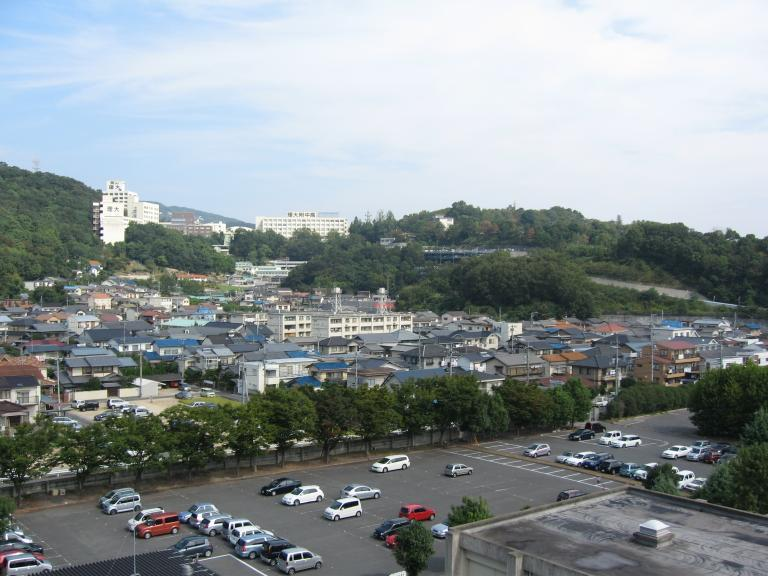
\includegraphics[bb=0 0 768 576,scale=.2]{../2/0.jpg}
\caption{変換前の元画像}
\end{minipage}
\begin{minipage}{0.3\hsize}
\center
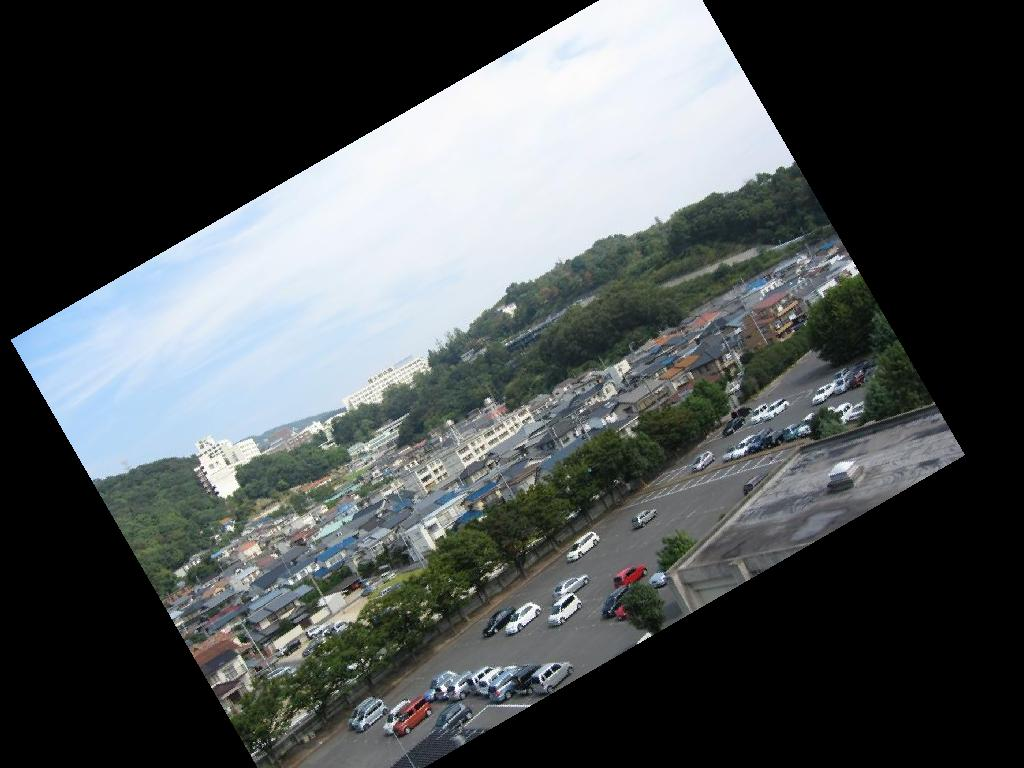
\includegraphics[bb=0 0 1024 768,scale=.13]{../2/outa.jpg}
\caption{行列aでの変換}
\end{minipage}
\begin{minipage}{0.3\hsize}
\center
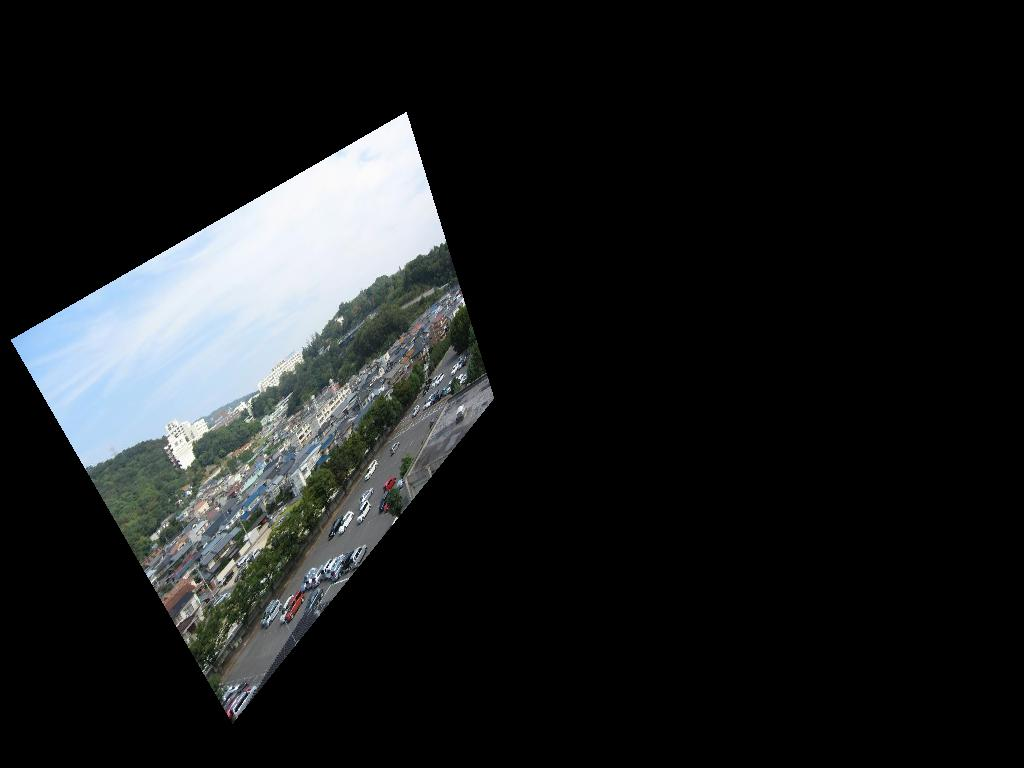
\includegraphics[bb=0 0 1024 768,scale=.13]{../2/outb.jpg}
\caption{行列bでの変換}
\end{minipage}
\end{tabular}
\end{figure}

どちらも画像の左上の位置は一致しており, 左上の点がy軸上の点として, xz平面で反時計回りに回転したような画像の変形になっている. 

\newpage
%%%%%%%%%%%%%%%%%%%%%%%%%%%%%%%%%%%%%%%%%%%%%%%%%%
\subsection{pano0.cについて}
%%%%%%%%%%%%%%%%%%%%%%%%%%%%%%%%%%%%%%%%%%%%%%%%%%
このプログラムでは, 同一視点から撮影された遠景の画像を射影変換によって重ね合わせ, 1枚のパノラマ画像のような画像を作り出すものである. 以下の行列m0d,m1dで変換した元画像と生成画像を示す. 

\begin{minipage}{0.5\hsize}
\begin{verbatim}

    double m0d[][3]={
      1,0,-100,
      0,1,-100,
      0,0,1
    };
\end{verbatim}
\end{minipage}
\begin{minipage}{0.5\hsize}
\begin{verbatim}

    double m1d[][3]={
       0.980063, 0.155844, -15.090362,
      -0.055756, 1.153389, -109.259360,
      -0.000139, 0.000316, 0.982279
    };
\end{verbatim}
\end{minipage}

\begin{figure}[htbp]
\begin{tabular}{ccc}
\begin{minipage}{0.3\hsize}
\center
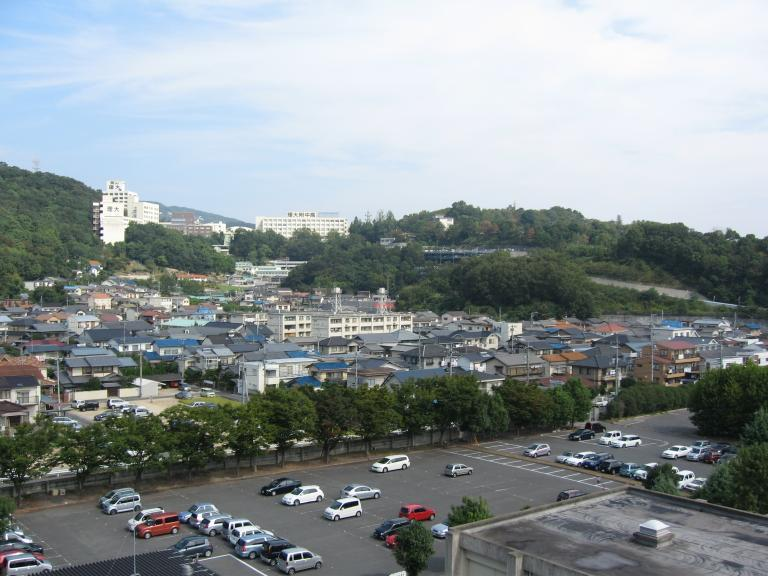
\includegraphics[bb=0 0 768 576,scale=.15]{../2/0.jpg}
\caption{行列m0dで変換する元画像1}
\end{minipage}
\begin{minipage}{0.3\hsize}
\center
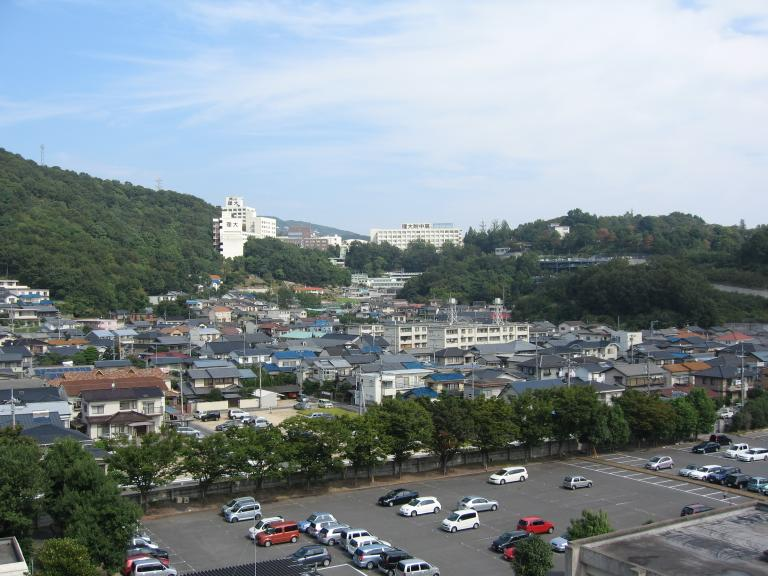
\includegraphics[bb=0 0 768 576,scale=.15]{../2/1.jpg}
\caption{行列m1dで変換する元画像2}
\end{minipage}
\begin{minipage}{0.4\hsize}
\center
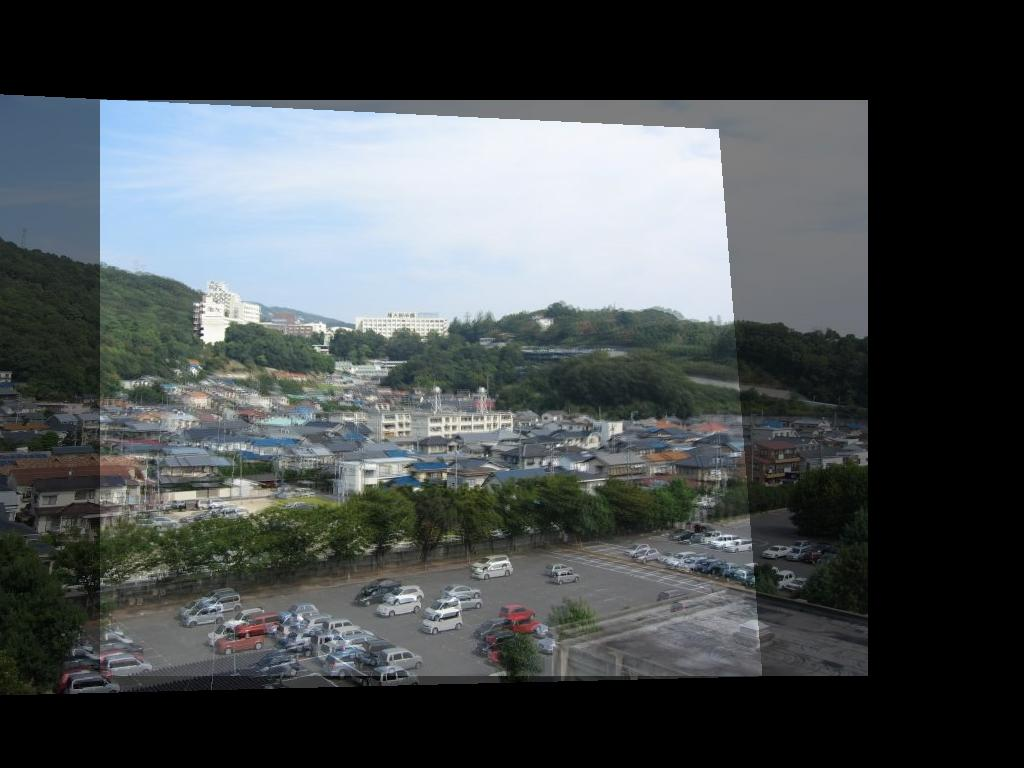
\includegraphics[bb=0 0 1024 768,scale=.15]{../2/panoout.jpg}
\caption{生成したパノラマ画像}
\end{minipage}
\end{tabular}
\end{figure}

%%%%%%%%%%%%%%%%%%%%%%%%%%%%%%%%%%%%%%%%%%%%%%%%%%
\subsection{pano0.cの改良}
%%%%%%%%%%%%%%%%%%%%%%%%%%%%%%%%%%%%%%%%%%%%%%%%%%
pano0.cではm0dの値が変わると二枚の画像が上手く重ねられない. 
そこでm1dの値はm0dと以下の行列m10の行列積をとるようにする.
\begin{verbatim}

    double m10[][3]={
      0.980063, 0.155844, 98.500361,
      -0.055756, 1.153389, 0.503900,
      -0.000139, 0.000316, 1
    }

\end{verbatim}

以下の関数で行列積を計算した. 
\begin{verbatim}

void mult33(double a[3][3],double b[3][3], double c[3][3]){
  int i,j,k;
  for(i=0;i<3;i++) {
    for(j=0;j<3;j++) {
      for(k=0;k<3;k++) {
	a[i][j]+=b[i][k]*c[k][j];
      }
    }
  }
}
\end{verbatim}

%%%%%%%%%%%%%%%%%%%%%%%%%%%%%%%%%%%%%%%%%%%%%%%%%%%%%%%%%%%%
\section{変換行列の算出/最小2乗法}
%%%%%%%%%%%%%%%%%%%%%%%%%%%%%%%%%%%%%%%%%%%%%%%%%%%%%%%%%%%%

%%%%%%%%%%%%%%%%%%%%%%%%%%%%%%%%%%%%%%%%%%%%%%%%%%
\subsection{概要}
%%%%%%%%%%%%%%%%%%%%%%%%%%%%%%%%%%%%%%%%%%%%%%%%%%
pano0.cで画像の変換を実装したが, この変換に用いられる射影行列はプログラムの処理の外側から引っ張ってきたものだった.
そこで合成する画像の4つの対応点からこの射影行列を作成するプログラムlsq.cを作成する.

%%%%%%%%%%%%%%%%%%%%%%%%%%%%%%%%%%%%%%%%%%%%%%%%%%
\subsection{lsq.cに現れる関数について}
%%%%%%%%%%%%%%%%%%%%%%%%%%%%%%%%%%%%%%%%%%%%%%%%%%
lsq.cはパノラマ画像で用いる似まいの画像の対応点からpano0.cで用いる変換行列を生成するプログラムである. lsq.cに現れる関数について説明する.

\begin{itemize}

\item {\bf Matrix}

  行列を管理する構造体.
  H, W: H × W 行列であることを表す.
  data: 要素を格納した double 型の配列.(i,j) 要素は data[i*W+j] に格納される.
\item {\bf Elem(Martix*mt, int i, int j);}

  行列 mt の (i,j) 要素の取得,および,代入に使う.
  s+=Elem(mt,i,j); や Elem(mt,i,j)=0; のような書式が可能.
\item {\bf double*Row(Matrix*mt, int i);}

  行列の第 i 行ベクトルを表すポインタを取得する.
  double*mi=Row(mt,i); を行った後は,mi[j] が Elem(mt,i,j) と同じ意味になる.ループの内
  側で,i が固定,j が変化する時には,一度ポインタを取得しておく方が良い.
\item {\bf Matrix*MatrixAlloc(int H, int W);}

  H×W 行列を作成する.確保された領域の値は未定義.
\item {\bf void MatrixClear(Matrix*mt);}

  行列の全て要素に 0 を代入する.
\item {\bf void MatrixCopy(Matrix*mtD, Matrix*mt);}
  
  行列 mt を mtD にコピーする.mtD は mt と同じ大きさで確保されている必要がある.
\item {\bf void MatrixCopyT(Matrix*mtD, Matrix*mt);}

  行列 mt の転置を mtD に代入する.mtD は正しく確保されている必要がある.
\item {\bf void MatrixMultT(Matrix*D, Matrix*A, Matrix*B);}

  D = AB T を計算する.D は確保されている必要がある.A と B の大きさが正しく対応している
  必要がある.
\item {\bf void MatrixPrint(Matrix*mt);}

  行列を stdout に出力する.
\item {\bf void MatrixQRDecompColMajor(Matrix*mtR, Matrix*mt);}

  mtを上三角行列と行直行行列に分解する.
  mtR は正しい大きさで確保されている必要がある.
\item {\bf void MatrixSimeqLr(Matrix*mtB, Matrix*mtR);}
  
  $mtBmtR^{-T}$を計算し, mtBを上書きする.
\end{itemize}

%%%%%%%%%%%%%%%%%%%%%%%%%%%%%%%%%%%%%%%%%%%%%%%%%%
\subsection{実行結果}
%%%%%%%%%%%%%%%%%%%%%%%%%%%%%%%%%%%%%%%%%%%%%%%%%%
以下の対応点でlsq.cを実行した.

\begin{minipage}{0.5\hsize}
\begin{verbatim}

xy[][2]={     // from 0.jpg
    111,212,
    169,354,
    454,455,
    451,221,
}

\end{verbatim}
\end{minipage}
\begin{minipage}{0.5\hsize}
\begin{verbatim}

uv[][2]={     // from 1.jpg
    230,227,
    287,365,
    573,467,
    568,231,
}

\end{verbatim}
\end{minipage}
実行結果は以下の様になった.
\begin{verbatim}
0.922122 0.007513 123.332960 -0.038207 0.960041 25.029107 -0.000106 -0.000000
\end{verbatim}
これに 1 を合わせた行列をm10としてpano0.cを実行し, 以下の画像が得られた.
\newpage
\begin{figure}[h]
\begin{tabular}{cc}
\begin{minipage}{0.5\hsize}
\center
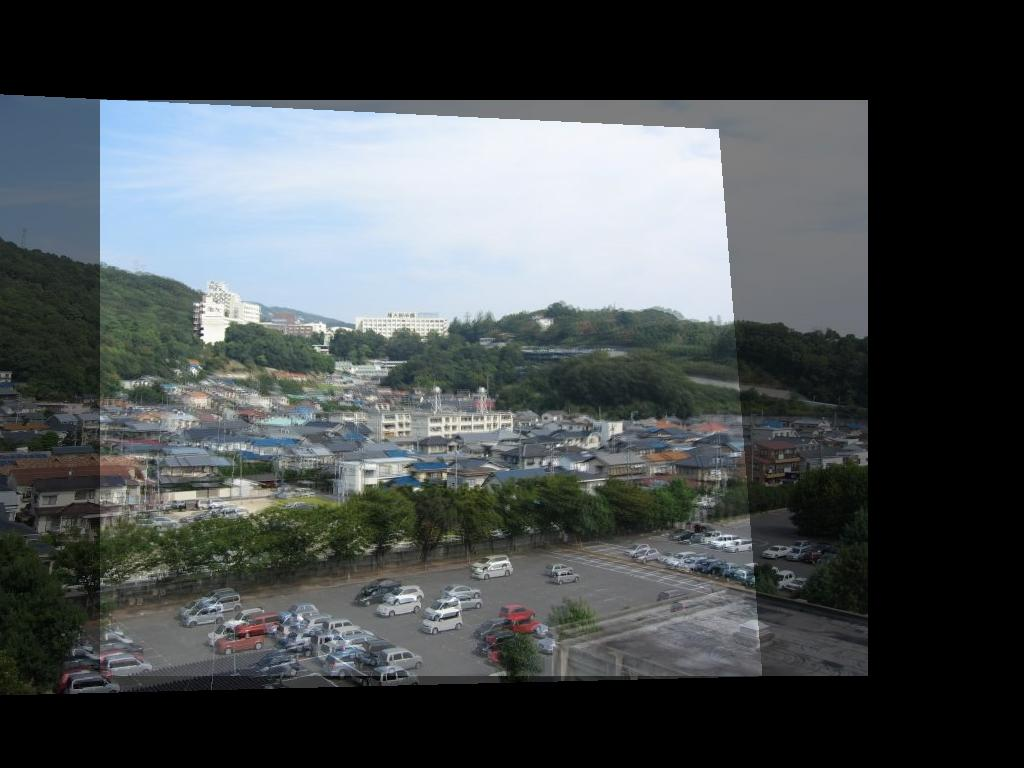
\includegraphics[bb=0 0 1024 768,scale=.2]{../2/panoout.jpg}
\caption{前回の出力画像}
\end{minipage}&
\begin{minipage}{0.5\hsize}
\center
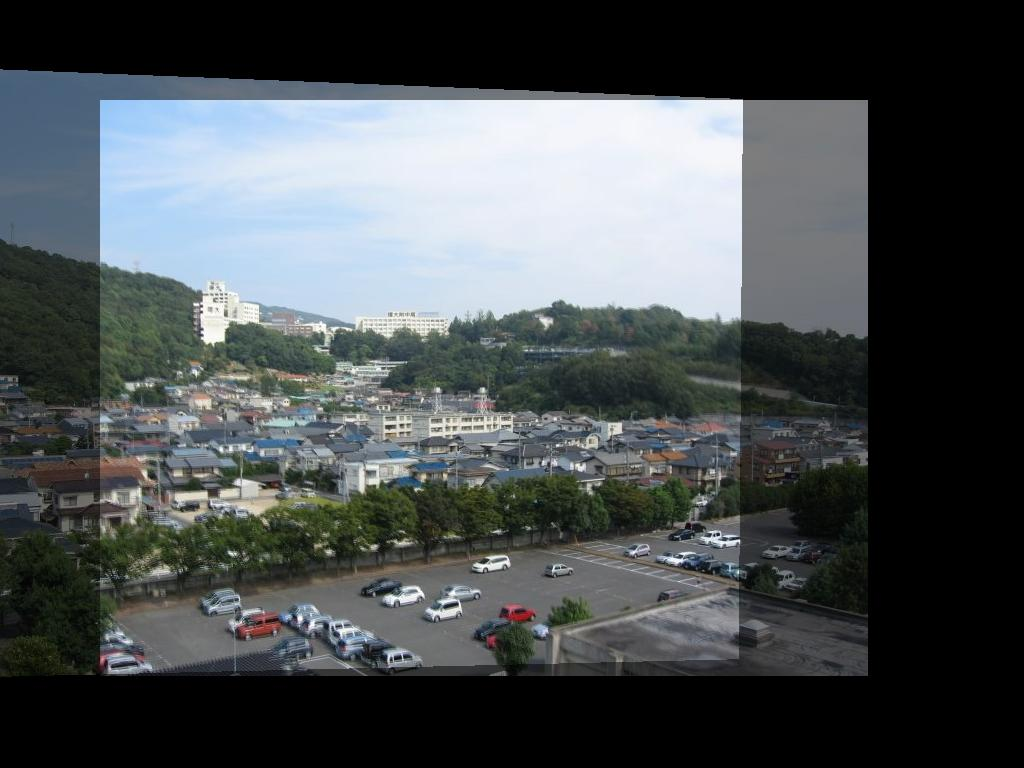
\includegraphics[bb=0 0 1024 768,scale=.2]{../3/out.jpg}
\caption{選んだ対応点から得られた行列を使用した出力画像}
\end{minipage}
\end{tabular}
\end{figure}

前回よりパノラマ画像のクオリティが高くなっている.
これはlsq.cによるものでなく, よりよい対応点の選別によるものであり, 
実際の画像合成アルゴリズムは前回と同様である. 


%%%%%%%%%%%%%%%%%%%%%%%%%%%%%%%%%%%%%%%%%%%%%%%%%%%%%%%%%%%%
\section{特徴点の自動検出 1}
%%%%%%%%%%%%%%%%%%%%%%%%%%%%%%%%%%%%%%%%%%%%%%%%%%%%%%%%%%%%
%%%%%%%%%%%%%%%%%%%%%%%%%%%%%%%%%%%%%%%%%%%%%%%%%%
\subsection{概要}
%%%%%%%%%%%%%%%%%%%%%%%%%%%%%%%%%%%%%%%%%%%%%%%%%%
画像の特徴点を自動検出させるためにTKfilter.cを作成する.
計算部であるImageFeature()を完成させ, 可能であればその計算を最適化させる. 

%%%%%%%%%%%%%%%%%%%%%%%%%%%%%%%%%%%%%%%%%%%%%%%%%%
\subsection{ImageFeature()の作成}
%%%%%%%%%%%%%%%%%%%%%%%%%%%%%%%%%%%%%%%%%%%%%%%%%%
以下のようなコードを作成した.

\begin{verbatim}
 void ImageFeature(Matrix*im2,Image*im){
  int x,y,u,v,W=7,ix,iy;
  double a;
  for(y=W+1;y<im->H-W-1;y++) for(x=W+1;x<im->W-W-1;x++){
    double ixx,ixy,iyy;
    ixx=iyy=ixy=0;
    for(v=-W;v<=W;v++) for(u=-W;u<=W;u++){
      ix=IElem(im, x+u+1, y+v, 1) - IElem(im, x+u-1, y+v, 1);
      iy=IElem(im, x+u, y+v+1, 1) - IElem(im, x+u, y+v-1, 1);
      ixx+=ix*ix;
      ixy+=ix*iy;
      iyy+=iy*iy;
    }
    a=((ixx+iyy)-sqrt(pow(ixx+iyy,2)-4*(ixx*iyy-pow(ixy,2))))/2;
    DElem(im2,x,y)=a; // 実際には [ixx,ixy;ixy,iyy] の小さい方の固有値を入れる.
  }
}
\end{verbatim}

出力結果は以下である.
\begin{center}
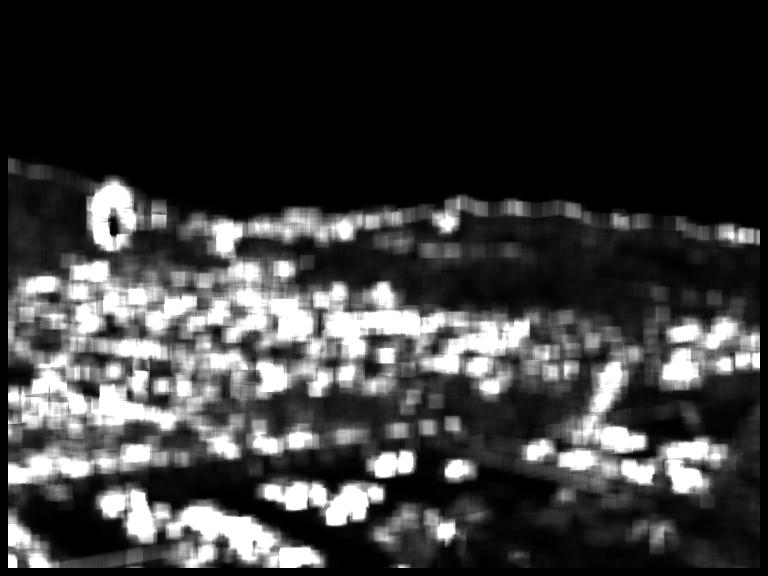
\includegraphics[bb=0 0 768 576,scale=.35]{../4/out.jpg}
\end{center}
このプログラムでは特徴点検出に多くの計算時間を要してしまう. 
そのため, その計算部の効率化が望まれる. 
そこで, その計算に対してGPUによる処理を適用した. 
以下はそのコードである. 
{\baselineskip 2mm
\begin{verbatim}
#include"image.h"
#define getpix(x,y) img[((x)+imW*(y))*3+1]

__global__ void gpuTK_vertical(float*tmp,unsigned char *img,int imW,int imH){
  int x=blockDim.x*blockIdx.x+threadIdx.x;
  int y=blockDim.y*blockIdx.y+threadIdx.y;
  int v,W=7;
  int mat=imW*imH;

  if(W+1<=y && y<imH-W-1)
    if(1<=x && x<imW-1){
      float ix,iy,ixx,ixy,iyy;
      ixx=iyy=ixy=0;
      for(v=-W;v<=W;v++){
	ix=getpix(x+1,y+v)-getpix(x-1,y+v);
	iy=getpix(x,y+v+1)-getpix(x,y+v-1);
	ixx+=ix*ix;
	ixy+=ix*iy;
	iyy+=iy*iy;
      }
      tmp[(x+imW*y)]=ixx;
      tmp[(x+imW*y+mat)]=ixy;
      tmp[(x+imW*y+mat*2)]=iyy;
    }
}

__global__ void gpuTK_horizontal(double*fimg,float*tmp,int imW,int imH){
  int x=blockDim.x*blockIdx.x+threadIdx.x;
  int y=blockDim.y*blockIdx.y+threadIdx.y;
  int u,W=7;
  int mat=imW*imH;

  if(W+1<=y && y<imH-W-1 &&
     W+1<=x && x<imW-W-1){
      float ixx,ixy,iyy;
      double lamd;
      ixx=iyy=ixy=0;
      for(u=-W;u<=W;u++){
	ixx+=tmp[(x+u+imW*y)];
	ixy+=tmp[(x+u+imW*y+mat)];
	iyy+=tmp[(x+u+imW*y+mat*2)];
      }
      lamd=((ixx+iyy)-sqrt(pow(ixx+iyy,2)-4*(ixx*iyy-ixy*ixy)))/2;
      fimg[x+imW*y]=lamd;
    }else fimg[x+imW*y]=0;
}


typedef struct {
  double *data;
  int W,H;
} Matrix;

// TKfilter.c では ImageFeature 本体を除去して,
// プロトタイプ宣言 void ImageFeature(Matrix*im2,Image*im); のみを書く.

extern "C"
void ImageFeature(Matrix*im2,Image*im){
  double*d_dst;
  float *d_tmp;
  unsigned char*d_src;
  cudaMalloc(&d_src,im->W*im->H*3);
  cudaMalloc(&d_dst,sizeof(double)*im->W*im->H);
  cudaMalloc(&d_tmp,sizeof(float)*im->W*im->H*3);
  cudaMemcpy(d_src,im->data,im->W*im->H*3,cudaMemcpyHostToDevice);
  gpuTK_vertical<<<dim3((im->W+15)/16,(im->H+15)/16),dim3(16,16)>>>(d_tmp,d_src,im->W,im->H);
  gpuTK_horizontal<<<dim3((im->W+15)/16,(im->H+15)/16),dim3(16,16)>>>(d_dst,d_tmp,im->W,im->H);  
  cudaMemcpy(im2->data,d_dst,im->W*im->H*sizeof(double),cudaMemcpyDeviceToHost);
  cudaFree(d_dst);
  cudaFree(d_src);
  cudaFree(d_tmp);
}
\end{verbatim}
}

これを適用したことにより, 特徴点検出にかかる計算時間は以下の様に改善された. 

\begin{tabular}{|l|c|c|}
  \hline
  & 改善前(GPU不使用の単純処理) & 改善後(GPUによる処理を採用)\\
  \hline
  時間 & 242 msec & 4.3 msec\\
  \hline
\end{tabular}

%%%%%%%%%%%%%%%%%%%%%%%%%%%%%%%%%%%%%%%%%%%%%%%%%%%%%%%%%%%%
\section{特徴点の自動検出 2}
%%%%%%%%%%%%%%%%%%%%%%%%%%%%%%%%%%%%%%%%%%%%%%%%%%%%%%%%%%%%

%%%%%%%%%%%%%%%%%%%%%%%%%%%%%%%%%%%%%%%%%%%%%%%%%%
\subsection{概要}
%%%%%%%%%%%%%%%%%%%%%%%%%%%%%%%%%%%%%%%%%%%%%%%%%%
TKfilterのMatrixLocalMaxを実装し, ImageFeatureで得られる特徴点指標画像の極大値を探し, その座標を配列に記録するプログラムを実装する. 
得られた配列を降順にソートすることで適した任意の数の特徴点を扱うことができる. 
また, ソートアルゴリズムは挿入ソートを採用した.

%%%%%%%%%%%%%%%%%%%%%%%%%%%%%%%%%%%%%%%%%%%%%%%%%%
\subsection{MatrixLocalMaxの実装}
%%%%%%%%%%%%%%%%%%%%%%%%%%%%%%%%%%%%%%%%%%%%%%%%%%
ImageFeatureで得られる特徴点指標画像の極大値を探し, その座標を配列に記録するプログラムを実装する. 
得られた配列を降順にソートすることで適した任意の数の特徴点を扱うことができる. 
また, ソートアルゴリズムは挿入ソートを採用した. 

\begin{verbatim}
int MatrixLocalMax(int w[][2], Matrix*im2){
  int x,y,u,v,W=7,n=0,a;
  int i,j;
  int tmp[2],t;
   for(y=W+1;y<im2->H-W-1;y++) for(x=W+1;x<im2->W-W-1;x++){
       double max=-1;
       for(v=-W;v<=W;v++) for(u=-W;u<=W;u++){
	   // (x,y) を中心とする 15x15 の矩形領域内で DElem(im2,x+u,y+v) の最大値を探す.
	   if(max<DElem(im2,x+u,y+v)) max = DElem(im2,x+u,y+v);
	 }
       // 最大値が DElem(im2,x,y) と等しいなら,(x,y) を特徴点として記録する.
       if(max==DElem(im2,x,y)){
	 a=n++; w[a][0]=x; w[a][1]=y;
	 for(i=0;i<n;i++){
	   t=DElem(im2,w[i][0],w[i][1]);
	   tmp[0]=w[i][0]; tmp[1]=w[i][1];
	   for(j=i;j>=1 && DElem(im2,w[j-1][0],w[j-1][1])<t;j--){
	     w[j][0]=w[j-1][0]; w[j][1]=w[j-1][1];
	   }
	   w[j][0]=tmp[0]; w[j][1]=tmp[1];
	 }
       }
     }
   //for(i=0;i<n;i++)printf("%f\n",DElem(im2,w[i][0],w[i][1]));
   return n; // 記録した点の数
}
\end{verbatim}
上位30個の特徴点を出力した結果は以下である. 
\begin{center}
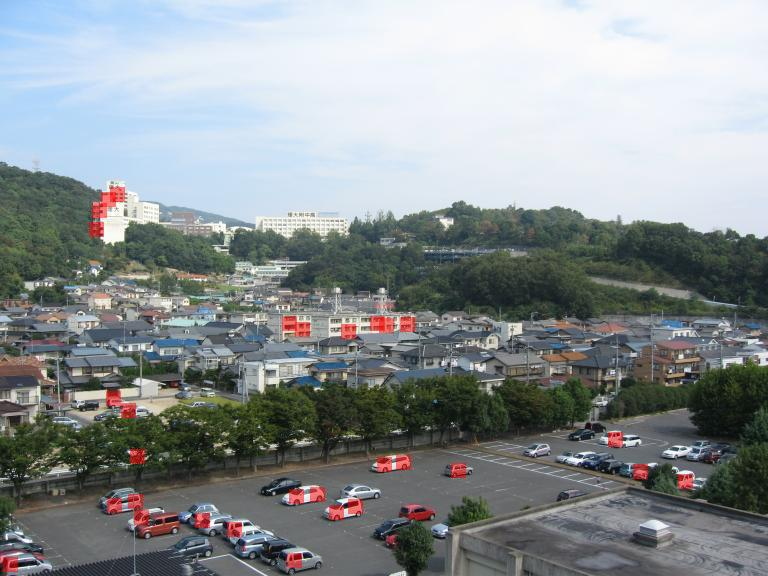
\includegraphics[bb=0 0 768 576,scale=.35]{../5/out2.jpg}
\end{center}

%%%%%%%%%%%%%%%%%%%%%%%%%%%%%%%%%%%%%%%%%%%%%%%%%%%%%%%%%%%%
\section{貪欲法による自動対応付け}
%%%%%%%%%%%%%%%%%%%%%%%%%%%%%%%%%%%%%%%%%%%%%%%%%%%%%%%%%%%%

%%%%%%%%%%%%%%%%%%%%%%%%%%%%%%%%%%%%%%%%%%%%%%%%%%
\subsection{概要}
%%%%%%%%%%%%%%%%%%%%%%%%%%%%%%%%%%%%%%%%%%%%%%%%%%
パノラマ画像の自動生成を行うには,両方の画像の同じ物体上に出現している特徴点を自動で探し出す必要がある.
この際,第1画像の第i特徴点と第2画像の第j特徴点が似ているかどうかを判定する.
このための最も簡単な類似度尺度はSum of Squared Differencesである.
即ち,特徴点周辺の小領域の画像を高次元ベクトルで表し,高次元空間のユークリッドノルムで画像の類似度を測る.
類似度の高い特徴点対を4組以上選ぶことで,正しい変換行列の算出が可能となる.

%%%%%%%%%%%%%%%%%%%%%%%%%%%%%%%%%%%%%%%%%%%%%%%%%%%
\subsection{greedy.cの作成}
%%%%%%%%%%%%%%%%%%%%%%%%%%%%%%%%%%%%%%%%%%%%%%%%%
特徴点の対応付けプログラムgreedy.cを作成する.
このプログラムには, TKfilter.cで得た特徴点座標を使用するため, 
これをgreedy.cで使用するためにファイルへ出力するコードを追加しておく.

準備として, 出力された二つの画像とそれらの画像の特徴点座標を用い, 一方の画像の特徴点一点が他方の画像の特徴点全ての点それぞれに対して特徴点が似ているかどうかの計算を一方の画像の特徴点全てに実行し, それを行列の構造体へ格納する.

行列式は以下のようになる. (ただし, double型の値を100000で割り, int型にキャストした値を表示するため, 実際に使用した値とは異なる)

{\baselineskip 2mm
  \scriptsize
\begin{verbatim}
  56  84  73  79  88  78  68  64  59  67  45  72  77  72  71  77  69  80  61  88  75  90  75  47  57  38  75  60  71  58
  53  84  70  71  60  62  58  62  70  54  61  73  63  65  69  68  65  43  47  78  58  69  88  51  44  47  70  60  64  38
  78  83  11  51  85  41  35  54  64  52  59  50  83  52  66  55  38  60  52  90  49  52  63  68  43  51  93  47  40  48
  66  80  49  46  45  51  40  60  49  37  60  39  93  48  57  56  53  63  44  75  44  45  44  61  42  45  80  40  54  43
  89 114  91  74   7  80  71  80  71  33 100  69 114  60  74  71  98  69  59  92  56  60  81  85  64  75  99  73  86  55
  78  99  35  10  70  49  22  71  71  46  66  57 110  58  76  66  64  70  65 111  51  49  73  84  53  64 106  53  57  40
  69  75  40  44  68  41  43  65  41  56  58  44  94  50  71  48  53  63  53  73  36  44  46  56  45  51 101  30  42  45
  72 102  40  28  53  47  13  62  61  41  69  57 102  59  73  67  67  67  61  97  45  54  68  71  52  56  89  60  64  33
  78  78  42  51  72  13  36  50  54  65  62  69  73  48  53  61  59  52  52  50  35  57  73  66  45  56  77  46  38  36
  74  74  53  60  43  63  44  64  59  16  56  21  95  47  68  52  47  56  39  84  41  46  56  49  37  44  90  47  51  44
  85  64  54  65  60  67  52  76  65  32  59   2 110  43  73  49  48  54  46  85  39  39  58  52  31  54 102  38  48  59
  63  42  76 102 107  67  88  82  66  81  30  70  54  49  68  63  50  50  42  47  56  82  73  37  58  39  63  43  56  66
  64  69  65  61  72  51  64  57   9  62  57  63 109  45  64  42  82  78  70  66  43  48  37  52  46  67 130  32  47  59
  51  64  65  75  90  45  58  46  46  76  47  80  48  68  48  67  63  66  44  46  49  81  64  40  61  41  58  49  50  51
  86  71  62  60  71  66  72  99  52  60  71  49 144  33  89  33  82  67  74  88  41  29  44  86  46  87 157  30  53  75
  51  56  59  77  85  58  58  43  62  56  38  62  46  62  47  63  38  51  35  66  49  66  66  33  40   5  48  47  47  38
  84  67  97  98  74  67  83  63  78  73  80  84  63  57  53  74  72  58  43  50  48  79  91  60  65  58  61  60  62  59
  63  58  65  61  82  68  74  78  48  52  54  51 114  46  74  21  80  65  59  86  43  32  39  56  45  78 141  27  51  68
  84  60 101 121 101  55 102  74  67 102  74 100  66  56  63  85  79  72  52   8  59  95  85  59  79  64  60  61  62  74
  87  75  98 131 140  77 108  68 105 114  68 128   6  97  62 109  62  69  45  69  87 125 132  63  86  53  45  82  73  73
  63  51  49  50  53  54  47  52  41  37  42  33  90  38  46  33  41  40  52  77  30  33  54  39   8  40  87  34  37  45
  75  47  44  62  80  34  61  52  44  54  53  46  76  37  44  30  41  40  39  57  29  30  58  50  29  52  91  22   4  55
  54  65  48  51  54  59  48  58  44  34  51  31  98  46  65  27  51  45  49  91  35  29  47  46  24  42 103  34  43  40
  53  37  77  97  91  64  79  65  59  69  38  61  48  63  46  56  49  51  40  49  50  75  71  19  44  34  61  46  47  64
  52  71  67  69  32  60  60  51  66  29  57  61  56  52  50  56  53  47  25  60  44  57  66  49  46  34  51  51  56  34
  69  40  45  54  85  49  54  63  51  55  35  46  77  46  41  46  41  54  55  74  36  39  67  41  18  50  95  37  31  57
  71  47  50  59  76  49  67  70  42  53  54  45  99  30  57  24  67  52  46  61  30  26  43  52  39  70 122  17  28  64
  65  81  40  43  58  40  34  49  57  45  57  60  64  53  60  67  40  60  38  73  43  62  67  54  44  35  62  53  53  11
  60  57  39  37  60  48  36  60  43  40  37  35  93  37  50  34  44  47  55  80  29  29  46  46  18  42  94  32  37  43
  66  74  47  63  72  38  41  48  61  55  58  57  60  56  56  69  40  53  37  59  48  64  66  54  42  27  49  47  43  29

\end{verbatim}
}

第一画像の第(行数)番目の特徴点と第二画像の第(列数)番目の特徴点のSSD(差の二乗和)が30点$×$30点$=$900点格納される. 
この行列の値は小さいものほど対応する特徴点二点が一致している可能性が高いといえる. 
そのためgreedy.cでもっとも重要とされるのはこの行列中の値で小さいものを探索し, 第一画像の特徴点と第二画像の特徴点をうまく対応させる処理である. 
その処理として, 以下の様な方法を実装した.

\begin{itemize}
\item{方法1}

第一画像で特徴点らしさの高い点から第二画像の特徴点との対応を決定する. 
処理手順としては, 上記の様な行列の一番上の行から一行ずつその行の中で一番値の小さな点を探索し, 第一画像の行数番目の特徴点と第二画像の列数番目の特徴点が対応すると決定する. 

行列の決定した点の列の値に無限値を格納し, それ以降の探索で同じ点を採用しないようにする. 
実行結果の特徴点の対応セットは30セット中12セットが一致していた.
特徴点をより正確に一致させるために次の様な方法を採用した.

\item{方法2}

行列の中の値全てを探索し, 一番値の小さい値の対応点を決定とする.
対応点が決まるとその点の行と列の値に無限値を格納し, それ以降の処理で同じ点を取らない様にする. 
実行結果は30セット中19セットが実際に一致していた. 
\end{itemize}

\subsection{問題と改善案}
今回作成したgreedy.cでは方法1で取り組んだ場合も方法2で取り組んだ場合も現状30個の特徴点を全て正確に対応させられていない.
しかし, この問題はgreedy.cだけでの問題ではない. greedy.cの入力ファイルである0.feaと2.feaに記された座標はそれぞれ30点であるが, 一方の特徴点が他方の画像中にあるとは限らないのである. そのため, いくらgreedy.cの性能を向上させても30点全てを正確に対応させることは物理的に不可能なのである. 

\begin{itemize}
\item{改善案1}

TKfilter.cから出力される特徴点を100個にするなど, 余分に多く特徴点を出力する. 
これにより, 多くの特徴点の中から対応する特徴点のセットを考えることができ, greedy.cで指定する特徴点セットの数が少ないほどその指定した数の特徴点セットの信頼性が高くなり, また今回の30点で試行する場合でも方法2よりもよい結果になることが期待できる. 
しかし, 方法1,方法2では扱う行列が大きくなればなるほど処理が重くなるため, 余分に取る点の個数は最適なものを考えて決めなければならない.

\item{改善案2}

TKfilter.cから出力される一方の画像の特徴点座標を他方の画像中にあるもののみとする条件を加える. 
これによりgreedy.cが捌く行列は大きくならないため, 処理の軽量化が期待できる. 
ただしこの方法では, 一方の画像中の点が他方の画像中にあるかないかを判断できることが前提である. 

\end{itemize}

改善案1を採用し, 方法2で特徴点対応付けを実装すると, 選んだ特徴点30セットが全て一致した. 


%%%%%%%%%%%%%%%%%%%%%%%%%%%%%%%%%%%%%%%%%%%%%%%%%%%%%%%%%%%%
\section{RANSACによる自動対応付け}
%%%%%%%%%%%%%%%%%%%%%%%%%%%%%%%%%%%%%%%%%%%%%%%%%%%%%%%%%%%%

%%%%%%%%%%%%%%%%%%%%%%%%%%%%%%%%%%%%%%%%%%%%%%%%%%
\subsection{概要}
%%%%%%%%%%%%%%%%%%%%%%%%%%%%%%%%%%%%%%%%%%%%%%%%%%
前章ではTKfilter.cで得られた二つの画像の特徴点を対応付けするプログラムを作成した. 
今回はそのプログラムから得られた特徴点セットから4セットを選び, 二つの画像を合成するのに適切な射影行列を計算するプログラムを作成する. 
どの4点を選ぶとよいかを判断することは難しいので, ランダムに選んだ4点で行列の適正を計算することを繰り返して最も適した行列を採用する.

%%%%%%%%%%%%%%%%%%%%%%%%%%%%%%%%%%%%%%%%%%%%%%%%%%
\subsection{作成過程}
%%%%%%%%%%%%%%%%%%%%%%%%%%%%%%%%%%%%%%%%%%%%%%%%%%
ファイルを新たに作成せずgreedy.cを拡張して射影行列の計算と選出を実装した. 
TKfilter.cから特徴点の対応セット30をファイルに出力し, そのファイルをgreedy.cで参照する形をとった. 
その対応点のセットから無作為に4つ拾うアルゴリズムは, 以下の様にした. 
\begin{enumerate}
\item 特徴点セットをすべてw[30][4]に格納する.
\item 0から29までの数が1つずつ格納された配列rndAry[30]の中の値を無作為に入れ替える. 
\item rndAry[0],rndAry[1],rndAry[2],rndAry[3]に格納された値を添字とする特徴点セットw[][]に格納された特徴点セットを採用する.
\end{enumerate}

選ばれた特徴点セットで射影行列を計算するが, これにより得られた射影行列は無作為に選ばれた特徴点によるものであるため, 適切な行列かどうかは判別ができない. そこで以下の様な計算で得られた値の大きさで判断する. 

\begin{enumerate}
\item w[][]に格納されたある特徴点セットをx,y,u,vとする
\item 一方の画像の特徴点座標x,yが画像の台形変換により他方の画像の特徴点座標u,vに近ければ制度の高い射影行列である可能性が高い
\item この座標x,yが変換後に移る座標と座標u,vの距離の2乗が一定の値より小さい場合カウントする
\item 30セット全てにこの操作をし, カウントした値を返す
\item この値の数が大きいほど使用した射影行列が適切であったことの証明となる
\end{enumerate}

以上の様な操作を次の様な手順でより最適な射影行列を計算する.

\begin{enumerate}
\item 対応付けられた特徴点から無作為に4セット選出する
\item それらから射影行列を計算する
\item 得られた射影行列の適正を図る
\item 得られたカウントがこれより前に得られたものより大きければこの射影行列を保持する
\item 指定した回数以上を繰り返し, 最も適した射影行列を出力する
\end{enumerate}

上記の手順が今回拡張したgreedy.cの中身になる.
また, 上記の通り, このプログラムではlsq.cの射影行列計算を頻繁に実行するため, lsq.c内のmain関数の関数名をLSQに変更し, greedy.cから使用できるように仕様の変更をした. 

得られた射影行列を用いて0.jpgと2.jpgを合成した画像は次のようになった.


\begin{figure}[h]
\begin{center}
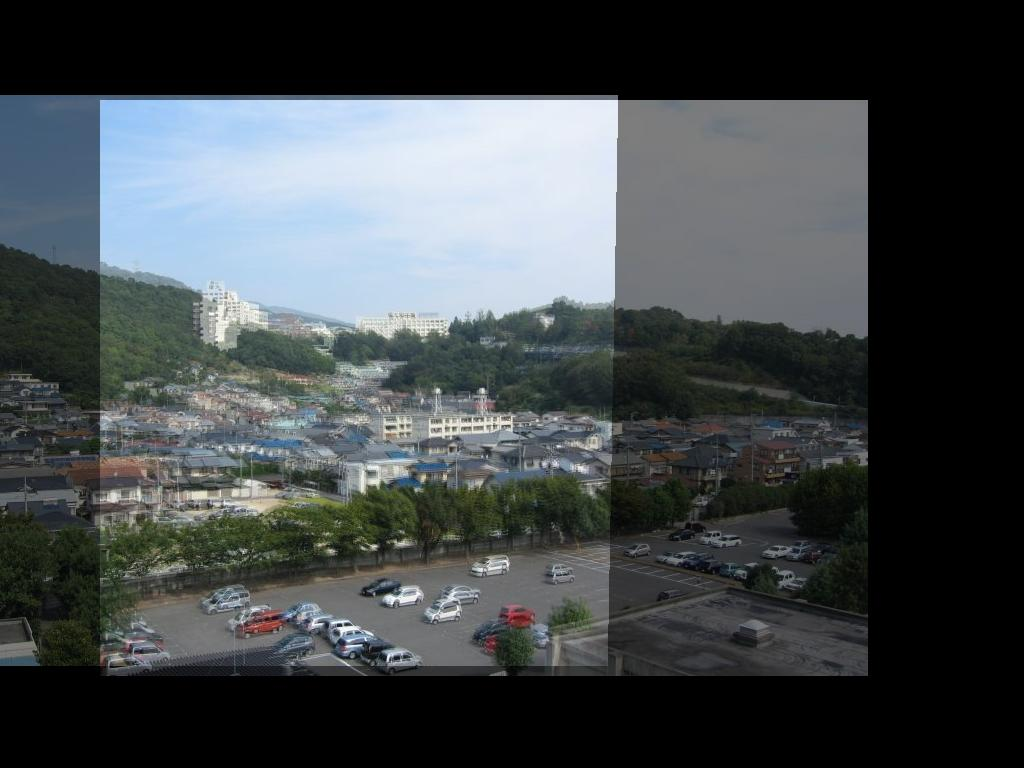
\includegraphics[bb=0 0 1024 768,scale=.3]{../7/out.jpg}
\caption{0.jpgと2.jpgの合成}
\end{center}
\end{figure}


%%%%%%%%%%%%%%%%%%%%%%%%%%%%%%%%%%%%%%%%%%%%%%%%%%%%%%%%%%%%
\section{まとめ}
%%%%%%%%%%%%%%%%%%%%%%%%%%%%%%%%%%%%%%%%%%%%%%%%%%%%%%%%%%%%

%%%%%%%%%%%%%%%%%%%%%%%%%%%%%%%%%%%%%%%%%%%%%%%%%%
\subsection{概要}
%%%%%%%%%%%%%%%%%%%%%%%%%%%%%%%%%%%%%%%%%%%%%%%%%%

これまで作成したプログラムを組み合わせ, 一回の実行で画像の入力からパノラマ画像の出力まで行うプログラムを作成する. 
これまで作成した.cのプログラムは以下である.
\begin{itemize}
\item image.c
\item TKfilter.c
\item greedy.c
\item lsq.c
\item pano0.c
\end{itemize}

これらのプログラムの内, TKfilter.c, greedy.c, pano0.cについて, ヘッダーファイルにして関数を使用するため, main関数を除いた部分をそれぞれTKfilter.h, greedy.h, pano.hにコピーした. 
lsq.cについては, 前章の時点でmain関数をそのまま関数として使うために関数名をLSQ関数に書き換えてある.

また, 3枚の画像の合成を試みる.

%%%%%%%%%%%%%%%%%%%%%%%%%%%%%%%%%%%%%%%%%%%%%%%%%%
\subsection{main.cの作成}
%%%%%%%%%%%%%%%%%%%%%%%%%%%%%%%%%%%%%%%%%%%%%%%%%%
これまで作成したプログラムを扱うmain.cを作成する.
中身はヘッダーファイルにしたプログラムTKfilter.c, greedy.c, pano0.cのmain関数の処理を変数の扱いに変更を加えながらそのまま引用するようにした. 
また, 3枚合成を実装するため, 今までの2枚合成の処理後にその合成画像と3枚目の画像を合成する処理を
加えた. 

次の実行での出力画像を示す.
\begin{verbatim}
./a.out 0.jpg 1.jpg 2.jpg
\end{verbatim}

\begin{figure}[h]
\begin{center}
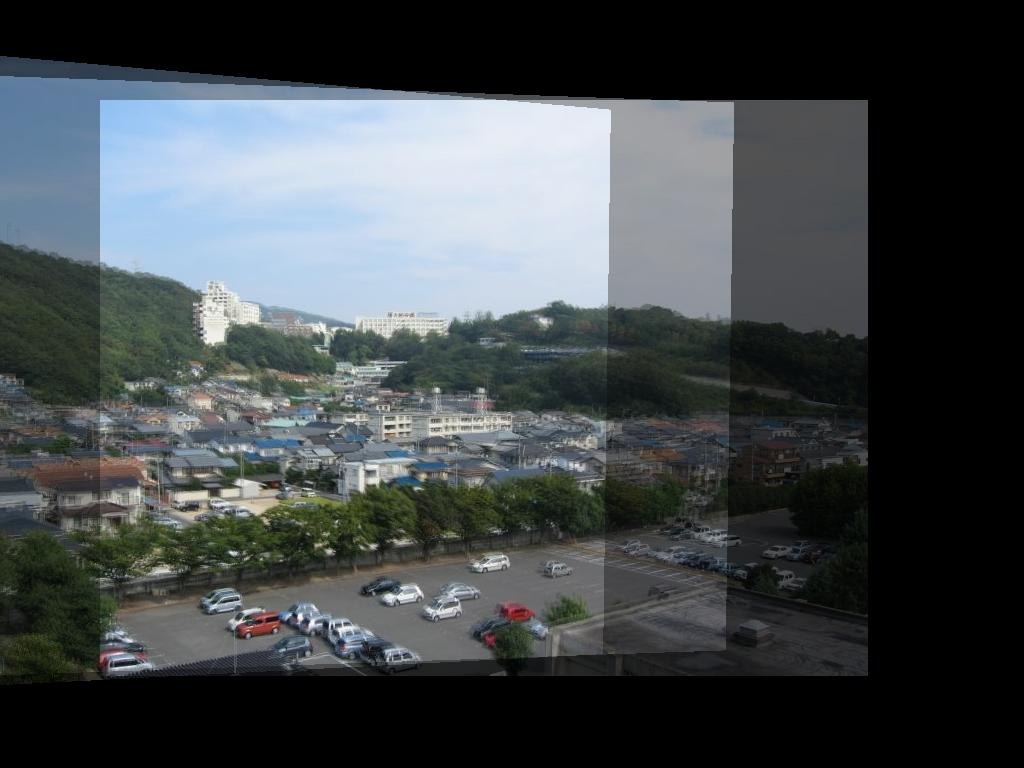
\includegraphics[bb=0 0 1024 768,scale=.3]{test.jpg}
\caption{0.jpg,1.jpg,2.jpgの合成}
\label{薄めない}
\end{center}
\end{figure}
\newpage
また, これまでの処理では画像の重なりがない部分は色が薄くなってしまう. 
そこで, 以下の様にpanoのImageImageProjectionAlphaの処理を改良した. 重なりのある部分は重なる色の値を足してその値に0.5を掛けたものを格納し, 重なりのない部分は色を薄くせずにそのままの値を格納するようにした.

{\baselineskip 2mm
\begin{verbatim}
改良前
      id->data[(y*id->W+x)*3+0] += is->data[(v*is->W+u)*3+0]*alpha,
      id->data[(y*id->W+x)*3+1] += is->data[(v*is->W+u)*3+1]*alpha,
      id->data[(y*id->W+x)*3+2] += is->data[(v*is->W+u)*3+2]*alpha;


改良後
      if(id->data[(y*id->W+x)*3+0]||
	 id->data[(y*id->W+x)*3+1]||
	 id->data[(y*id->W+x)*3+2]){
	id->data[(y*id->W+x)*3+0] = (id->data[(y*id->W+x)*3+0]+
				     is->data[(v*is->W+u)*3+0])*0.5,
	  id->data[(y*id->W+x)*3+1] = (id->data[(y*id->W+x)*3+1]+
				       is->data[(v*is->W+u)*3+1])*0.5,
	  id->data[(y*id->W+x)*3+2] = (id->data[(y*id->W+x)*3+2]+
				       is->data[(v*is->W+u)*3+2])*0.5;
      }else{
	id->data[(y*id->W+x)*3+0] = is->data[(v*is->W+u)*3+0],
	  id->data[(y*id->W+x)*3+1] = is->data[(v*is->W+u)*3+1],
	  id->data[(y*id->W+x)*3+2] = is->data[(v*is->W+u)*3+2];
      }

\end{verbatim}
}

改良後のコードで図\ref{薄めない}の画像を出力すると次の様になる.

\begin{figure}[h]
\begin{center}
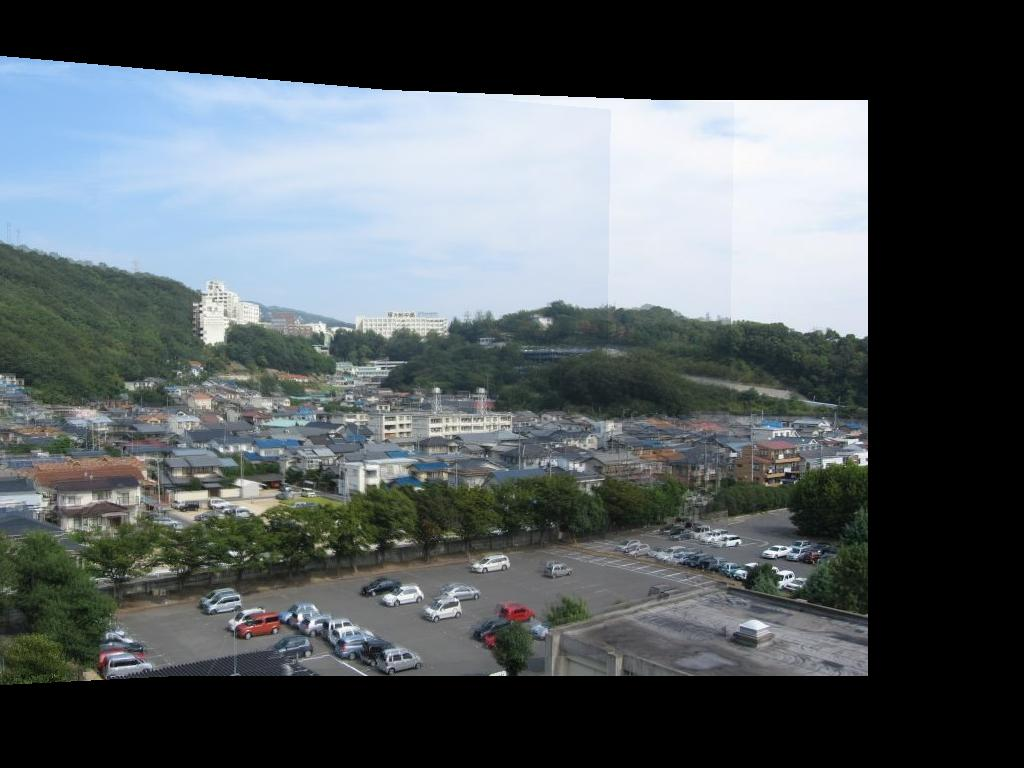
\includegraphics[bb=0 0 1024 768,scale=.4]{out012.jpg}
\caption{色を薄めない処理を採用}
\end{center}
\end{figure}



\end{document}
